\documentclass[12pt]{article}
\usepackage{fontspec}
\usepackage{amsmath}
\usepackage{amssymb}
\usepackage{geometry}
\usepackage{graphicx}
\usepackage[BoldFont, SlantFont, CJKchecksingle]{xeCJK}
\setCJKmainfont[BoldFont={WenQuanYi Micro Hei/Bold}]{WenQuanYi Micro Hei}
\geometry{left=1cm,right=1cm,top=2.5cm,bottom=2.5cm}


\title{数学笔记}
\author{Ying Kanyang\thanks{Ningbo Foreign Language School J1907}}

\begin{document}
  \maketitle{}
  \tableofcontents{}
  \newpage{}
  \section{笔记正文}
		\subsection{March 11, 2018}
			\subsubsection{题1,2004年全国赛题}
			已知点$A(0,3)$、$B(-2,-1)$、$C(2,-1)$,$P(t,t^{2})$为抛物线$y=x^{2}$上位于三角形ABC内(包括边界)的一动点,$BP$所在直线交$AC$于$E$,$CP$所在直线交$AB$于$F$。请将$\frac{BF}{CE}$表示为自变量$t$的函数。\\
			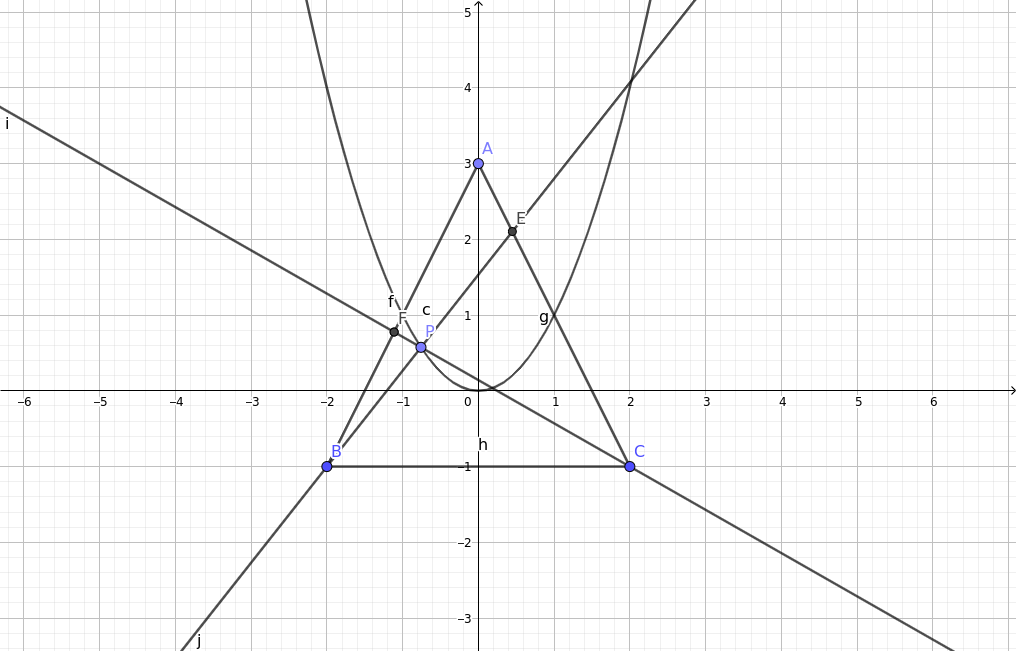
\includegraphics[scale=0.4]{pictures/2018-03-11-1-2004全国赛.png}
			\\
			思路:\\
			第一种方法就是直接解析,计算出点的坐标并求出$BF$与$CE$的长度,从而得出比值。但是这种方法需要深厚的代数功底,需要解出大量高次含参方程,不推荐在竞赛考试中使用。\\
			第二种方法借助了相似,通过相似将$\frac{BF}{CE}$转换为另一个可简单表示并化简的代数式。但是比较难想到。\\
			\\
			解法一:\\
			通过解析,得到下列直线的解析式:
			\begin{equation}
				\left\{
				\begin{aligned}
					AB&:y=2x+3\\
					AC&:y=-2x+3\\
					BP&:y=\frac{t^2+1}{t+2}x+\frac{2 t^2-t}{t+2}\\
					CP&:y=\frac{t^2+1}{t-2}x-\frac{2 t^2+t}{t-2}
				\end{aligned}
				\right.
			\end{equation}
			通过联立方程组的方式,得到$E(\frac{-2 t^2+4 t+6}{t^2+2 t+5},\frac{7 t^2-2 t+3}{t^2+2 t+5})$与$F(\frac{2 \left(t^2+2 t-3\right)}{t^2-2 t+5},\frac{7 t^2+2 t+3}{t^2-2 t+5})$\\
			用欧几里得算法得到$BF$与$CE$的线段长度:
			\begin{equation}
				\left\{
					\begin{aligned}
						BF&:\sqrt{\left.\left| \frac{7 t^2+2 t+3}{t^2-2 t+5}+1\right.\right| ^2+\left.\left| \frac{2 \left(t^2+2 t-3\right)}{t^2-2 t+5}+2\right.\right| ^2}\\
						CE&:\sqrt{\left.\left| \frac{7 t^2+2 t+3}{t^2-2 t+5}+1\right.\right| ^2+\left.\left| \frac{2 \left(t^2+2 t-3\right)}{t^2-2 t+5}+2\right.\right| ^2}
					\end{aligned}
				\right.
			\end{equation}
			化简\footnote{本步骤使用了Mathematica}得:
			\begin{equation}
				\left\{
					\begin{aligned}
						BF&:4 \sqrt{5} \left.\left| \frac{t^2+1}{t^2-2 t+5}\right.\right|\\
						CE&:4 \sqrt{5} \left.\left| \frac{t^2+1}{t^2-2 t+5}\right.\right|
					\end{aligned}
				\right.
			\end{equation}
			$\therefore{}\frac{BF}{CE}=\frac{t^{2}+2t+5}{t^{2}-2t+5}$ \footnote{$t^{2}+2t+5$与$t^{2}-2t+5$恒成立}\\
			\\
			解法二:\\
			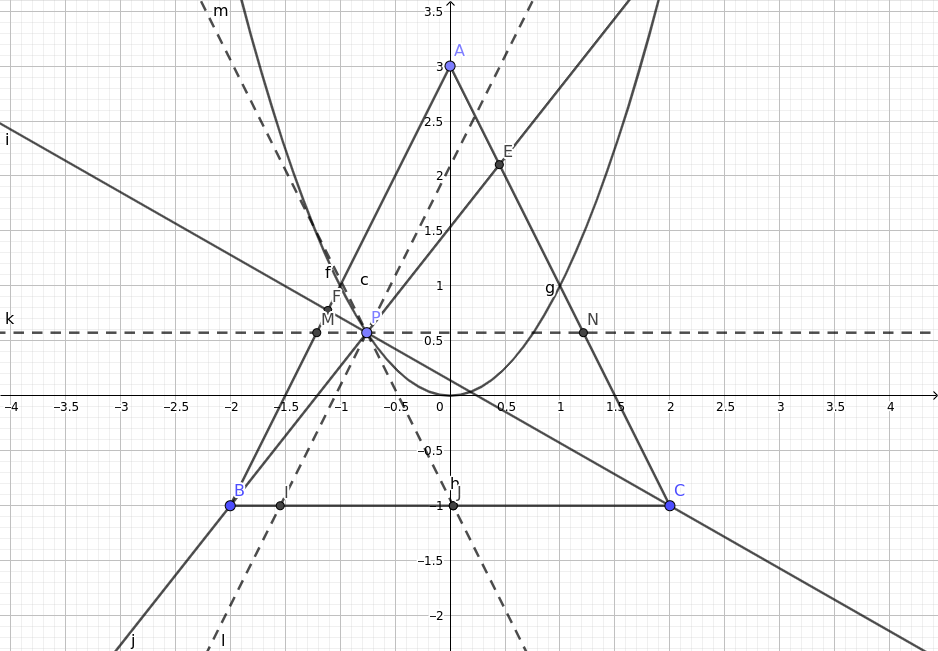
\includegraphics[scale=0.4]{pictures/2017-03-11-1-2004全国赛辅助线.png}\\
			过$P$作$BC$平行线交$AB$与$AC$于点$M$和$N$\\
			过$P$作$AB$平行线交$BC$于点$I$\\
			过$P$作$AC$平行线交$BC$于点$J$\\
			$\because{}MB=NC$\\
			$\therefore{}\begin{aligned}
    	\frac{BF}{CE}&=\frac{BF}{MB}\cdot\frac{CN}{CE}\\
    	&=\frac{BC}{CI}\cdot\frac{BJ}{BC}\\
    	&=\frac{BJ}{CI}\\
    	&=\frac{BC-PN}{BC-PM}\\
    	&=\frac{BC-(\frac{1}{2}MN-t)}{BC-(\frac{1}{2}MN+t)}
    \end{aligned}$\\
			代入$MN=3-t^{2}$与$BC=4$,可得$\frac{BF}{CE}=\frac{t^{2}+2t+5}{t^{2}-2t+5}$\\
			\\
			一般地,对于上述的解法,需要注意$P$的范围,通过求出抛物线与线段$AB$和$AC$的交点,得到范围$-1\leqslant{}t\leqslant{}1$
	\subsection{April 01, 2018}
		\subsubsection{题2,无来源}
			已知抛物线$y=x^2+(k+1)x+1$与$x$轴的两交点$A$、$B$不全在原点的左侧,抛物线顶点为$C$,则当$\Delta{}ABC$恰为等腰三角形时,求$k$的值。\\
			\\
			思路:\\
			讨论制约条件并进行解析。\\
			\\
			解:\\
			$\because{}$函数与$x$轴有两个交点\\
			$\therefore{}\Delta{}>0$\\
			$\therefore{}\begin{aligned}
				\Delta{}&=(k+1)^{2}-4\\
				&=k^{2}+2k+1-4\\
				&=k^{2}+2k-3\\
				&>0
			\end{aligned}$\\
			$\therefore{}k>3$或$k<-1$\\
			$\because{}$两交点$A$、$B$不全在原点的左侧且$x^2+(k+1)x+1=0$两根之积为$1$\\
			$\therefore{}A_{x}\cdot{}B_{x}=1$且$A$、$B$均在原点右侧\\
			$\therefore{}$\begin{equation}
				\left\{
					\begin{aligned}
						x_{1}\cdot{}x_{2}&>0\\
						x_{1}+x_{2}&>0\\
					\end{aligned}
				\right.
			\end{equation}\\
			$\begin{aligned}
				AB&=|x_{1}-x_{2}|\\
					&=\sqrt{(x_{1}-x_{2})^{2}}\\
					&=\sqrt{k^{2}+2k-3}\\
			\end{aligned}$\\
			作$CH\bot{}x$轴于点$H$\\
			可得$CH:AH=\sqrt{3}:1$\\
			进一步,推导出:\\
			\begin{equation}
				\begin{aligned}
					AH\cdot{}\sqrt{3}&=CH\\
					\frac{\sqrt{3[(k+1)^{2}-4]}}{2}&=\frac{(k+1)^{2}-4}{4}\\
				\end{aligned}
			\end{equation}
			令$(k+1)^{2}-4$为$\alpha{}$\\
			解得\begin{equation}
				\left\{
					\begin{aligned}
						\alpha{}_{1}&=0\\
						\alpha{}_{2}&=12\\
					\end{aligned}
				\right.
			\end{equation}\\
			对于$(k+1)^{2}-4=\alpha{}_{1}$,解得:\begin{equation}
				\left\{
					\begin{aligned}
						k_{1}&=1\\
						k_{2}&=-3\\
					\end{aligned}
				\right.
			\end{equation}\\
			对于$(k+1)^{2}-4=\alpha{}_{2}$,解得:\begin{equation}
				\left\{
					\begin{aligned}
						k_{3}&=3\\
						k_{4}&=-5\\
					\end{aligned}
				\right.
			\end{equation}\\
			$\because{}$制约条件\\
			$\therefore{}k=-3$或$-5$\\
			特殊的,当$k=-3$时,$A$、$B$、$C$三点重合,$\Delta{}ABC$不存在\\
			$\therefore{}k=-5$
\end{document}
